\chapter{Approximate inference}

\begin{description}
    \item[Stochastic simulation] \marginnote{Stochastic simulation}
        Class of methods that draw $N$ samples from the distribution
        and estimate an approximate posterior $\hat{\mathcal{P}}$.

        \begin{description}
            \item[$\delta$-stochastic absolute approximation] 
                Given $\delta \in ]0, 0.5[$ and $\varepsilon \in ]0, 0.5[$, a $\delta$-stochastic absolute approximation has error:
                \[ \left\vert \prob{X | \matr{E}} - \hat{\mathcal{P}}(X | \matr{E}) \right\vert \leq \varepsilon \]
                Moreover, the method might fail (with greater error) with probability $\delta$.

            \item[$\delta$-stochastic relative approximation] 
                Given $\delta \in ]0, 0.5[$ and $\varepsilon \in ]0, 0.5[$, a $\delta$-stochastic relative approximation has error:
                \[ \frac{\left\vert \prob{X | \matr{E}} - \hat{\mathcal{P}}(X | \matr{E}) \right\vert}{\prob{X | \matr{E}}} \leq \varepsilon \]
                Moreover, the method might fail (with greater error) with probability $\delta$.
        \end{description}

        \begin{theorem}
            Approximate inference is NP-hard for any $\delta, \epsilon < 0.5$.
        \end{theorem}

    \item[Consistency] \marginnote{Consistency}
        A sampling method is consistent if:
        \[ \lim_{N \rightarrow \infty} \hat{\mathcal{P}}(x) = \prob{x} \]
\end{description}



\section{Sampling from an empty network}
\marginnote{Sampling from an empty network}

Sample each variable in topological order (i.e. from parents to children).

The probability $\mathcal{S}$ of sampling a specific event $x_1, \dots, x_n$ is given by the
probability of the single events knowing their parents:
\[ \mathcal{S}(x_1, \dots, x_n) = \prod_{i=1}^n \prob{x_i | \texttt{parents}(X_i)} = \prob{x_1, \dots, x_n} \]

\begin{theorem}
    Sampling from an empty network is consistent.

    \begin{proof}
        Let $N$ be the number of samples and 
        $\mathcal{N}(x_1, \dots, x_n)$ the number of times the event $x_1, \dots, x_n$ has been sampled.
        \[
            \begin{split}
                \lim_{N \rightarrow \infty} \hat{\mathcal{P}}(x_1, \dots, x_n) &=
                \lim_{N \rightarrow \infty} \frac{\mathcal{N}(x_1, \dots, x_n)}{N} \\
                &= \mathcal{S}(x_1, \dots, x_n) = 
                \prob{x_1, \dots, x_n}
            \end{split}    
        \]
    \end{proof}
\end{theorem}

\begin{example}
    Given the following Bayesian network:
    \begin{center}
        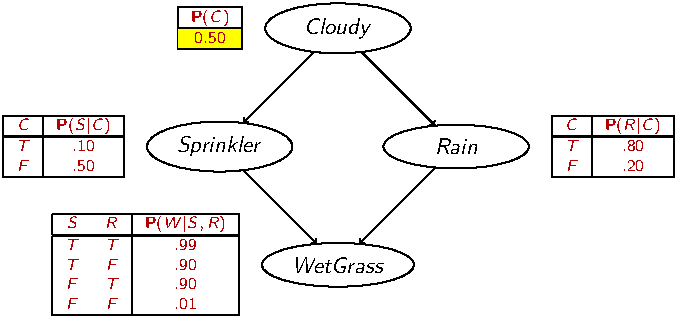
\includegraphics[width=0.5\textwidth]{img/_approx_infer_example.pdf}
    \end{center}
    
    A possible sampling order is \texttt{Cloudy}, \texttt{Sprinkler}, \texttt{Rain}, \texttt{WetGrass}.

    Assuming that a random generator gives the sequence of probabilities $(0.4, 0.8, 0.1, 0.5)$,
    the sample will be:
    \[ \langle \prob{C}, \prob{S | C}, \prob{R | C}, \prob{W | S, R} \rangle \]
    \[ \langle C=\texttt{false}, \prob{S | C=\texttt{false}}, \prob{R | C=\texttt{false}}, \prob{W | S, R} \rangle \]
    \[ \langle C=\texttt{false}, S=\texttt{false}, R=\texttt{true}, \prob{W | S=\texttt{false}, R=\texttt{true}} \rangle \]
    \[ \langle C=\texttt{false}, S=\texttt{false}, R=\texttt{true}, W=\texttt{true} \rangle \]

    Note that the adopted convention is the following: 
    if $r$ it the probability given by a random generator and $\prob{X} = p$, $X = \texttt{true}$ if $r \leq p$.
\end{example}



\section{Rejection sampling}
\marginnote{Rejection sampling}

Given a known evidence $\matr{E}$, rejection sampling works as sampling from an empty network
but removes any sample that does no agree with the evidence.

Obviously if $\prob{\matr{E}}$ is low, the majority of the samples will be discarded and 
more iterations are required to reach the desired number of samples.

\begin{theorem}
    Rejection sampling is consistent.

    \begin{proof}
        Let $\mathcal{N}(\matr{X})$ be the number of times the event $\matr{X}$ has been sampled.
        \[
            \begin{split}
                \hat{\mathcal{P}}(\matr{X} | \matr{E}) &= 
                \frac{\mathcal{N}(\matr{X}, \matr{E})}{\mathcal{N}(\matr{E})} \\
                &\approx \frac{\prob{\matr{X}, \matr{E}}}{\prob{\matr{E}}} =
                \prob{\matr{X} | \matr{E}}
            \end{split}    
        \]
        The approximation derives from the consistency of sampling from an empty network.
    \end{proof}
\end{theorem}



\section{Likelihood weighting}
\marginnote{Likelihood weighting}

Given a known evidence $\matr{E}$, likelihood weighting samples non-evidence variables and 
weights each sample by the likelihood of the evidence.

The probability $\mathcal{S}$ of sampling a specific event $\matr{Z}$ and evidence $\matr{E}$ is given by the
probability of the single events in $\matr{Z}$ knowing their parents:
\[ \mathcal{S}(\matr{Z}, \matr{E}) = \prod_{z_i \in \matr{Z}} \prob{z_i | \texttt{parents}(z_i)} \]

The weight of a sample $(\matr{Z}, \matr{E})$ is given by the
probability of the single events in $\matr{E}$ knowing their parents:
\[ \text{w}(\matr{Z}, \matr{E}) = \prod_{e_i \in \matr{E}} \prob{e_i | \texttt{parents}(e_i)} \]

\begin{theorem}
    Likelihood weighting is consistent.

    \begin{proof}
        The weighted sampling probability is given by:
        \[ 
            \begin{split}
                \mathcal{S}(\matr{Z}, \matr{E}) \cdot \text{w}(\matr{Z}, \matr{E})
                &= \prod_{z_i \in \matr{Z}} \prob{z_i | \texttt{parents}(z_i)} \cdot \prod_{e_i \in E} \prob{e_i | \texttt{parents}(e_i)} \\
                &= \prob{\matr{Z}, \matr{E}}
            \end{split}
        \]
        This is a consequence of the global semantics of Bayesian networks.
    \end{proof}
\end{theorem}

\begin{example}
    Given the following Bayesian network:
    \begin{center}
        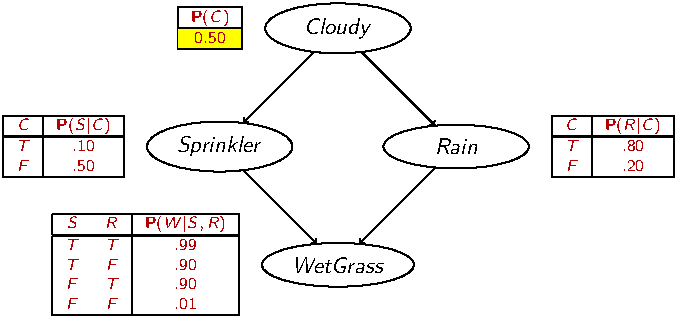
\includegraphics[width=0.5\textwidth]{img/_approx_infer_example.pdf}
    \end{center}

    Knowing that $S=\texttt{true}$ and $W=\texttt{false}$,
    we sample in the order: \texttt{Cloudy}, \texttt{Rain}.
    
    Assuming that a random generator gives the sequence of probabilities $(0.4, 0.1)$,
    the sample will be:
    \[ \langle \prob{C}, S=\texttt{true}, \prob{R | C}, W=\texttt{false} \rangle \]
    \[ \langle C=\texttt{true}, S=\texttt{true}, \prob{R | C=\texttt{true}}, W=\texttt{false} \rangle \]
    \[ \langle C=\texttt{true}, S=\texttt{true}, R=\texttt{true}, W=\texttt{false} \rangle \]

    The weight associated to the sample is given by the probability of the evidence:
    \[ 
        \begin{split}
            \text{w} &= \prob{S=\texttt{true} | C=\texttt{true}} \cdot \prob{W=\texttt{false} | S=\texttt{true}, R=\texttt{true}} \\
            &= 0.1 \cdot (1 - 0.99) = 0.001
        \end{split}
    \]
\end{example}



\section{Markov chain Monte Carlo}
\marginnote{Markov chain Monte Carlo}

Sampling on a Markov chain where states contain an assignment to all variables.

Adjacent states of the Markov chain differ by only one variable.
Therefore, the probability of an edge connecting two states is given by the probability of the updated variable known its Markov blanket:
\[ 
    \prob{x_i | \texttt{markov\_blanket}(X_i)} = 
    \prob{x_i | \texttt{parents}(X_i)} \cdot \prod_{Z_j \in \texttt{children}(x_i)} \prob{z_j | \texttt{parents}(Z_j)} 
\]

\begin{theorem}
    Markov chain Monte Carlo is consistent.

    Note: nevertheless, it is difficult to tell if convergence has been achieved.

    \begin{proof}
        Consequence of the fact that a long-run on a Markov chain converges to the posterior probability of the states.
    \end{proof}
\end{theorem}

\begin{description}
    \item[Compiled network]
        A naive implementation of Markov chain Monte Carlo requires to repeatedly compute the probabilities with the Markov blanket.
        A solution is to compile the network into a model-specific inference code.
\end{description}

\begin{example}
    Given the evidence $S=\texttt{true}$ and $W=\texttt{true}$,
    the structure of the Markov chain can be defined as follows:
    \begin{center}
        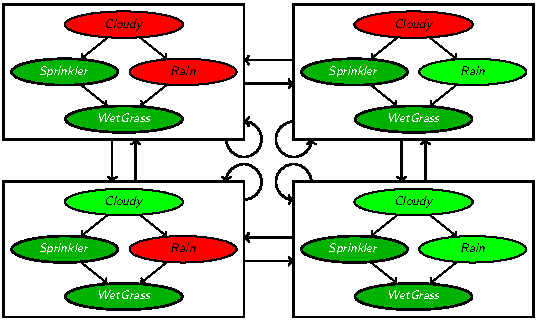
\includegraphics[width=0.5\textwidth]{img/_markov_chain_sampling.pdf}
    \end{center}
\end{example}